%*----------- SLIDE -------------------------------------------------------------
\begin{frame}[t]{Introdução} 
    \transdissolve[duration=0.5]
    Quando um robô móvel se move pelo meio ele pode sofrer problemas por não ter como usar sinais de GPS.

    Para solucionar esse problema frequentemente um robô móvel tem que estimar sua posição no espaço usando sensores e um mapa do ambiente.

    Para mapear um ambiente são utilizados principalmente dois tipos de mapas.
    %\newline
        \begin{columns}[t]
            \column{.05\linewidth}
            \column{.4\linewidth}
                \begin{enumerate}
                    \item \textit{elevation maps}
                    \item \textit{multi-level surface maps}
                \end{enumerate}
            \column{.6\linewidth}

        \end{columns}
%*----------- notes
    \note[item]{Notes can help you to remember important information. Turn on the notes option.}
\end{frame}
%-

%*----------- SLIDE -------------------------------------------------------------
\begin{frame}[t]{\textit{Elevation maps}} 
    \transdissolve[duration=0.5]
    A ideia por trás desse tipo de mapeamento é pegar $2\frac{1}{2}$ da informação sobre a altura dimensional armazenar em uma grade de duas dimensões e isso corresponderá a uma representação horizontal do meio.
    
    Tem como desvantagens:
    %\newline
        \begin{columns}[t]
            \column{.05\linewidth}
            \column{.4\linewidth}
                \begin{enumerate}
                    \item oferece um fraco suporte para a localização do robô;
                    \item mapeia apenas as superficies horizontal;
                    \item estruturas verticais não podem ser usadas para localização.
                \end{enumerate}
            \column{.6\linewidth}
            \begin{center}
            %\centerline{
                \begin{figure}
                    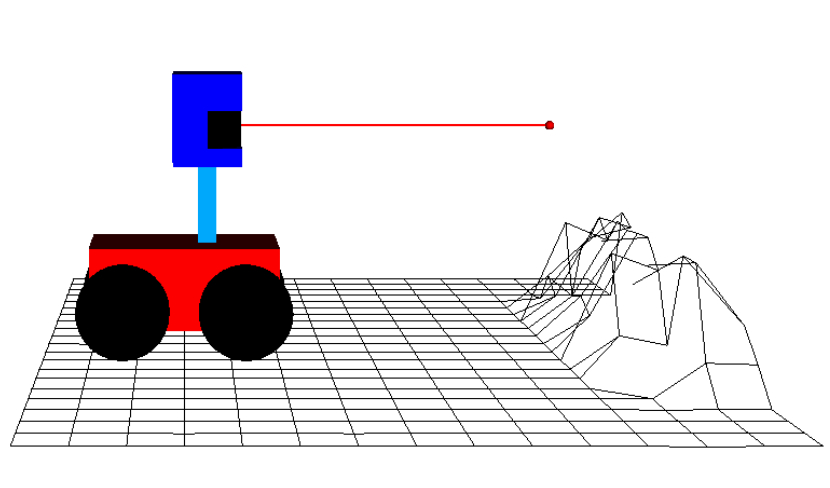
\includegraphics[width=0.5\textwidth]{elevation_map2.jpg}
                    \caption{Elevation maps\cite{article}}
                    % \roundpic[xshift=0cm,yshift=0cm]{2.5cm}{6cm}{pista}
                    %\caption{Pista de corrida \cite{agostini2007}}
                \end{figure}
            %}
            \end{center}
        \end{columns}
%*----------- notes
    \note[item]{Notes can help you to remember important information. Turn on the notes option.}
\end{frame}

%*----------- SLIDE -------------------------------------------------------------
\begin{frame}[t]{\textit{Multi-Level Surface maps}} 
    \transdissolve[duration=0.5]
    Veio para resolver os problemas do \textit{elevation map}
    
    Tem como características:
    %\newline
        \begin{columns}[t]
            \column{.05\linewidth}
            \column{.4\linewidth}
                \begin{enumerate}
                    \item ser uma extensão do \textit{elevation map};
                    \item representam intervalos que correspondem aos objetos verticais;
                    \item podem representar diversos níveis.
                \end{enumerate}
            \column{.6\linewidth}
            \begin{center}
            %\centerline{
                \begin{figure}
                    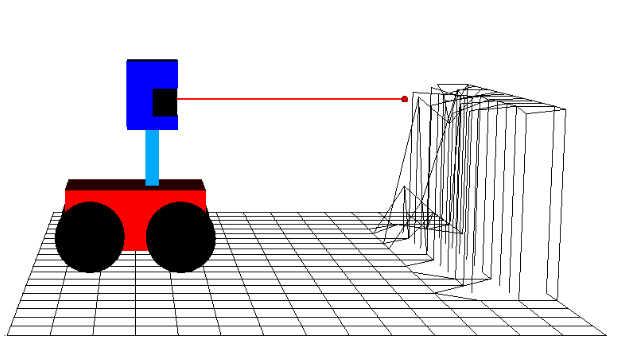
\includegraphics[width=1\textwidth]{mls.jpg}
                    \caption{Multi-level surface\cite{article}}
                    % \roundpic[xshift=0cm,yshift=0cm]{2.5cm}{6cm}{pista}
                    %\caption{Pista de corrida \cite{agostini2007}}
                \end{figure}
            %}
            \end{center}
        \end{columns}
%*----------- notes
    \note[item]{Notes can help you to remember important information. Turn on the notes option.}
\end{frame}

%-
%*----------- SLIDE -------------------------------------------------------------
\begin{frame}[c]{Objetivo} 
    % \framesubtitle{sub-objetivo}
    \transdissolve[duration=0.5]
   
    \begin{center}
        \Wider{%
        \begin{shaded}
        \begin{center}
            \vspace*{0.5cm}
            \resizebox{!}{0.35cm}{%
                \color{bg} Usar o \textit{multi-level surface map} para localização em ambientes externos.
            }%
        \end{center}
        \end{shaded}
        }%
    \end{center}
    
\end{frame}

